\documentclass[11pt,a4paper]{article}
\usepackage[utf8]{inputenc}
\usepackage[T1]{fontenc}
\usepackage{amsmath}
\usepackage{amsfonts}
\usepackage{amssymb}
\usepackage[left=3.0cm, right=3.0cm, top=3.0cm, bottom=3.0cm]{geometry}
\usepackage{xcolor}
\usepackage{graphicx}
\usepackage{caption}
\usepackage{subcaption}

% include code listings
\usepackage{listings}

% Defining colors for syntax highlighting
\definecolor{codegreen}{rgb}{0,0.6,0}
\definecolor{codegray}{rgb}{0.5,0.5,0.5}
\definecolor{codepurple}{rgb}{0.58,0,0.82}
\definecolor{backcolour}{rgb}{0.95,0.95,0.92}

\lstdefinestyle{mystyle}{
	backgroundcolor=\color{backcolour},   
	commentstyle=\color{codegreen},
	keywordstyle=\color{magenta},
	numberstyle=\tiny\color{codegray},
	stringstyle=\color{codepurple},
	basicstyle=\ttfamily\scriptsize,
	breakatwhitespace=false,         
	breaklines=true,                 
	captionpos=b,                    
	keepspaces=true,                 
	numbers=left,                    
	numbersep=5pt,                  
	showspaces=false,                
	showstringspaces=false,
	showtabs=false,                  
	tabsize=2
}

\lstset{style=mystyle}
\captionsetup[lstlisting]{font={scriptsize}}

% header and footer
\usepackage{fancyhdr}
\pagestyle{fancy}
\fancyhf{}
\lhead{Michele Guadagnini}
\rhead{\today}
\lfoot{Ex 10 - Quantum Information and Computing 2020/2021}
\rfoot{Page \thepage}

\author{Michele Guadagnini - ID 1230663}
\title{\textbf{Exercise 10 \\ Real Space Renormalization Group}}
\date{\today}

%File names must include your name, exercise number and codewords REPORT, and CODE.
%Example: Ex2-Rossi-REPORT.pdf
%The maximum length of the report is five pages
\begin{document}
\maketitle

\vspace{20pt}
\begin{abstract}
	The aim of this exercise is to compute the ground state of a 1D lattice of spin particles in a transverse field by mean of the Real Space Renormalization Group method. The obtained results are compared to the analytical Mean Field solution.
\end{abstract}

\section{Theory} %Explain briefly the theory you have based your solution on.
The system to be studied is the same of the previous exercise, 1D Ising model with transverse field with nearest neighbor interaction. The Hamiltonian is:
\begin{equation}
	H = \lambda \sum_{i=1}^{N} \sigma_{z}^{i} + \sum_{j=1}^{N-1} \sigma_{x}^{j} \sigma_{x}^{j+1} 
	\label{eq:ham}
\end{equation}
In this assignment we will use the \textit{Real Space Renormalization Group} method (RSRG) to compute the ground state of the system in the thermodynamical limit ($N \rightarrow \infty$).

RSRG is based on the physical hypothesis that the ground state of the whole system is composed only by the lowest-energy states of the system's non-interacting bipartitions.
In this way, starting from a system of a size that allows us to easily computes its eigenstates, it is possible to iteratively double the number of particles represented by the Hamiltonian while keeping low the computational cost, as the Hamiltonian size remains the same through all the iterations.

Starting from a system with $N$ particles the first step consists in building the initial Hamiltonian matrix $H_{in}$ of size $2^N$. Then the matrix is diagonalized and the algorithm proceeds repeating the following three steps:
\begin{itemize}
	\item the matrix is projected into a reduced space by using the matrix $P$ composed by the first $m$ eigenvalues; the same projection is applied also to the interaction terms.
	\begin{equation} \label{eq:proj}
	\begin{aligned}
		\widetilde{H_m} &= P^\intercal H_{in} P \\
		\widetilde{H_{left}} &= P^\intercal H_{left} P \\
		\widetilde{H_{right}} &= P^\intercal H_{right} P \\
	\end{aligned}	
	\end{equation} 
	\item the matrix of size $2^{2m}$ is created by padding the projected Hamiltonian and by computing the interaction term. In formula ($\otimes$ denotes the \textit{kronecker product} between two matrices):
	\begin{equation}
		\widetilde{H_{2m}} = \widetilde{H_m} \otimes \mathbb{I}_m + \mathbb{I}_m \otimes \widetilde{H_m} + \widetilde{H_{left}} \otimes \widetilde{H_{right}}
		\label{eq:doubleham}
	\end{equation}
	\item the matrix is diagonalized in order to get the new ground state and the projector for the next iteration.
\end{itemize}

Finally, we compare the obtained energy densities with the Mean Field analytical solution, that is:
\begin{equation}
	e_{MF}(\lambda) = 
	\begin{cases}
		-1 - \frac{\lambda^2}{4} & \quad \mbox{if } \lambda \in [-2;2] \\
		-|\lambda|               & \quad \mbox{if } \lambda \notin [-2;2] \\
	\end{cases}
\end{equation}


\section{Code Development} %Introduce strategies, tests, and report debugging problems, compilations options

\subsection{Design and Implementation}
A lot of the functions and subroutines needed to solve this problem have been already implemented for the previous assignment. Only some mathematical tools has been added to the module contained in the file \textit{Ex10-Guadagnini-RSRG-CODE.f90}. 
In Listing \ref{lst:kronprod} the implementation of the kronecker product. The module defines also the operator interface for this operation as \textit{\textbf{.kron.}}

\lstinputlisting[language=FORTRAN, firstnumber=124, linerange={124-148}, caption=Kronecker product between two matrices., label=lst:kronprod]{Ex10-Guadagnini-RSRG-CODE.f90}

The main effort of this work has been to build up the RSRG algorithm in the main program contained in the file \textit{Ex10-Guadagnini-CODE.f90} (see Listing \ref{lst:rsrg}). 
The loop contains the three steps explained in the Theory section and an additional portion of code that decides when to stop the iterations. A parameter representing the minimum improvement in the last step needed to continue the computation has been defined; it is called $ExitTh$ and can be changed by editing the configuration file. Also a maximum number of iterations has been set.

\lstinputlisting[language=FORTRAN, firstnumber=99, linerange={99-155}, caption=RSRG loop implementation., label=lst:rsrg]{Ex10-Guadagnini-CODE.f90}

A Python script (\textit{Ex10-Guadagnini-Script-CODE.py}) has been created in order to run the program over different parameters. A set of values between $0$ and $3$ has been used for $\lambda$, some values for $N$ and $m$ has been tested, while $ExitTh$ has been set to $5 \times 10^{-16}$, which is close to machine precision with DOUBLE numbers. 
This script has the capability to capture the output of the FORTRAN program, by setting the variable $verbosity$ to $false$, in order to limit the printings on the screen.
Also a Gnuplot script has been used to produce the results plots.

Finally, a second Python script (\textit{Ex10-Guadagnini-MeanField-CODE.py}) has been created to implement the Mean Field solution and use it as a comparison. 

\subsection{Debug and Test}
The program has been compiled and executed with the following commands:
\begin{lstlisting}[language=BASH,numbers=none]
	gfortran *CODE.f90 -o RGIsing1D.x -lblas -llapack -g -fcheck=all -Wall
	./RGIsing1D.x
\end{lstlisting}

To check the correctness of the code the results of the RSRG algorithm for systems with few particles have been compared to the exact solution obtained in the previous assignment.

\section{Results} %Present data and explain your results.

The algorithm has been run with several values for the input parameters. In particular, its behavior has been explored with different sizes of the initial system (parameter "NN") and different sizes of the matrix during iteration (parameter "TruncN"). 
The results are reported in Figure \ref{fig:gsall}. It can be seen that there are no significant differences in the energy densities obtained. 

\begin{figure}%[h]
	\centering
	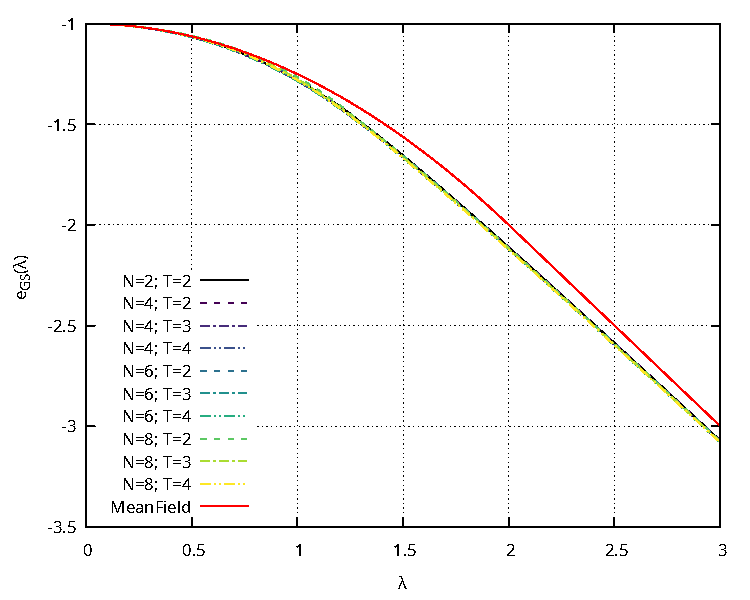
\includegraphics[width=0.95\linewidth]{Plots/GroundStatesAll.pdf}
	\caption{Energy densities of all the computed solutions. Also the Mean Field results are reported.}
	\label{fig:gsall}
\end{figure}

There is a small region around $\lambda$ = 1, where we know that the system has a phase transition, where they differ slightly more between each other. 
Anyway, the curves are not well overlapping in any region of the $\lambda$ space, except for $\lambda$ = 0; this could be due to numerical error.
Comparing the RSRG solutions with the Mean Field energy density, we can see that, while the solutions are equal for low $\lambda$ values, they start to separate again around $\lambda$ = 1. 
Indeed, we know that the Mean Field method predicts the phase transition at $\lambda$ = 2 and the greater difference between the two methods is found to be at $\lambda \sim 1.8$, as can be seen in Figure \ref{fig:gsdiff}.

\begin{figure}
	\centering
	\begin{subfigure}{0.49\textwidth}
		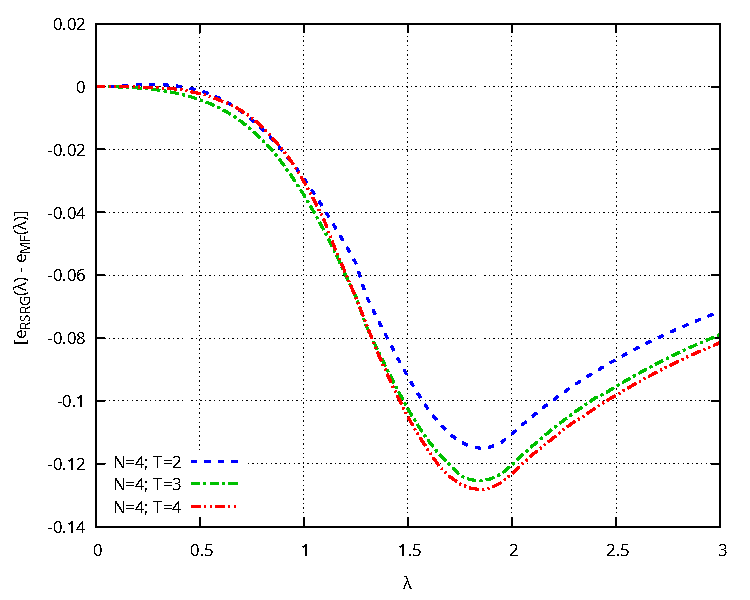
\includegraphics[width=1\linewidth]{Plots/GS_diff_N4.pdf}
		\caption{Same N, different T.}
		\label{fig:gsdiffN4}
	\end{subfigure}%
	\hfill
	\begin{subfigure}{0.49\textwidth}
		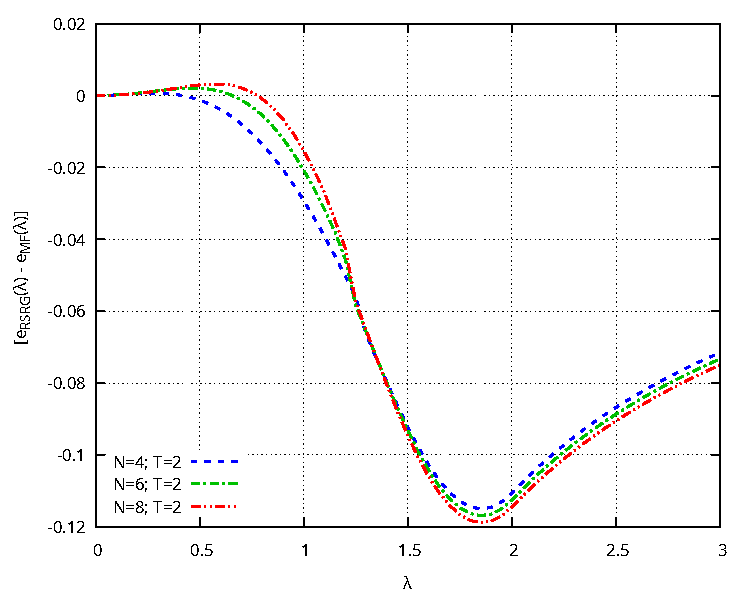
\includegraphics[width=1\linewidth]{Plots/GS_diff_T2.pdf}
		\caption{Same T, different N.}
		\label{fig:gsdiffT2}
	\end{subfigure}
	\caption{Difference between the energy densities of the RSRG results and the Mean Field solution. N represents the initial system size, while T is the iteration size.}
	\label{fig:gsdiff}
\end{figure}


\section{Self-evaluation} %What have you learned? What can be done next? What went wrong and why?

The Real Space Renormalization Group is a powerful method to estimate the energy density of the ground state of a spin system in thermodynamical limit. 
The method presents slightly different results for different initial or iteration sizes, especially around the phase transition region.
An interesting point not discussed here is the comparison with the Infinite Density Matrix Renormalization Group technique.

	
\end{document}
